\documentclass{article}

% if you need to pass options to natbib, use, e.g.:
\PassOptionsToPackage{numbers, compress}{natbib}
% before loading neurips_2019

% ready for submission
% \usepackage{neurips_2019}

% to compile a preprint version, e.g., for submission to arXiv, add add the
% [preprint] option:
%     \usepackage[preprint]{neurips_2019}

% to compile a camera-ready version, add the [final] option, e.g.:
\usepackage[schoolpaper]{neurips_2019}

% to avoid loading the natbib package, add option nonatbib:
%     \usepackage[nonatbib]{neurips_2019}

\usepackage[utf8]{inputenc} % allow utf-8 input
\usepackage[T1]{fontenc}    % use 8-bit T1 fonts
\usepackage{hyperref}       % hyperlinks
\usepackage{url}            % simple URL typesetting
\usepackage{booktabs}       % professional-quality tables
\usepackage{amsfonts}       % blackboard math symbols
\usepackage{nicefrac}       % compact symbols for 1/2, etc.
\usepackage{microtype}      % microtypography
\usepackage{graphicx}

\graphicspath{{images/}} 
\bibliographystyle{unsrtnat}

\title{Forecasting daily COVID-19 spread in regions around the world.}

% The \author macro works with any number of authors. There are two commands
% used to separate the names and addresses of multiple authors: \And and \AND.
%
% Using \And between authors leaves it to LaTeX to determine where to break the
% lines. Using \AND forces a line break at that point. So, if LaTeX puts 3 of 4
% authors names on the first line, and the last on the second line, try using
% \AND instead of \And before the third author name.

\author{%
  Frank Lawrence Nii Adoquaye Acquaye\thanks{http://acquayefrank.github.io} \\
  Faculty of Computer Science\\
  National Research University Higher School of Economics\\
  \texttt{fakvey@edu.hse.ru} \\
  % examples of more authors
  \And
  Bense Valerie Caroline \\
  Faculty of Computer Science\\
  National Research University Higher School of Economics\\
   \texttt{vbense@edu.hse.ru} \\
  % \AND
  % Coauthor \\
  % Affiliation \\
  % Address \\
  % \texttt{email} \\
  % \And
  % Coauthor \\
  % Affiliation \\
  % Address \\
  % \texttt{email} \\
  % \And
  % Coauthor \\
  % Affiliation \\
  % Address \\
  % \texttt{email} \\
}

\begin{document}

\maketitle

\begin{abstract}

\end{abstract}

\section{Problem statement:}
The year 2020 will forever be remembered as the year the earth stood still. This is  primarily due to the spread of \href{https://en.wikipedia.org/wiki/Coronavirus_disease_2019}{COVID-19}. As Data Scientists we seek to provide solutions to problems facing humanity and the world at large. In this regard we seek to develop a forecasting model that will predict the daily spread of COVID-19 in regions around the world.  Our model predicts the number of daily new cases in regions around the world in order to help policy makers plan and manage the COVID-19 pandemic.  

\section{Dataset summary and EDA:}

\subsection{Background of dataset:}
The White House Office of Science and Technology Policy (OSTP) pulled together a coalition of research groups and companies (including Kaggle) to prepare the \href{https://www.kaggle.com/allen-institute-for-ai/CORD-19-research-challenge}{COVID-19 Open Research Dataset (CORD-19)} to attempt to address \href{https://www.kaggle.com/allen-institute-for-ai/CORD-19-research-challenge/tasks}{key open scientific questions on COVID-19}. Those questions are drawn from \href{https://www.nationalacademies.org/event/03-11-2020/standing-committee-on-emerging-infectious-diseases-and-21st-century-health-threats-virtual-meeting-1}{National Academies of Sciences, Engineering, and Medicine’s (NASEM)} and the \href{https://www.who.int/blueprint/priority-diseases/key-action/Global_Research_Forum_FINAL_VERSION_for_web_14_feb_2020.pdf?ua=1}{World Health Organization (WHO)}.

\subsection{Data sources:}
The sources of data used in this project can be obtained from \href{https://www.kaggle.com/c/covid19-global-forecasting-week-5/overview}{Kaggle Dataset}.
Furthermore we choose to enrich the dataset with data on the population in the different countries. Data such as population density, percentage of urban population and median age.
This data was obtained from \href{https://www.kaggle.com/tanuprabhu/population-by-country-2020}{Kaggle} aswell. 


\subsection{Actual data:}
Since the accuracy of such a model is dependent on the freshness of the data, the most up to date data can be found \href{https://www.kaggle.com/c/covid19-global-forecasting-week-5/overview}{here}

\subsection{Actual data used in project:}
In this project we use frozen dataset i.e dataset that has been frozen in time and this dataset can be found \href{https://github.com/acquayefrank/MLDM2020-Project/tree/master/data}{here}

\subsection{Basic exploratory data analysis:}
The dataset for training consists of $8$ primary variables with a total of $914232$ line items. $1.6\%$  of the line items contained missing data. \emph{Figure 1} shows the a preview of the first five line items in training dataset.  Upon further investigations we realise that most instances had $Country = NaN$, also $Province\_State = Nan$ except in cases where the $Country\_Region = U.S.A$. For this reason we exempted these two variables or attributes. In the exploratory stage, there is no clear description of the weight parameter, but we may experiment with it, to see how it impacts predictions but most likely we may drop it. 
\\
\\
 \emph{Figure 2} shows the first five rows of the data for testing. One can easily realise that the target value was not supplied, for this reason we will drop the test dataset and split our training dataset in a manner that allows us to test our models.
 \\
 \\
 We split our training data into \emph{confirmed cases} and  \emph{fatalities}. This can be confirmed from  \emph{Figure 3}. 
 A simple summary statistic of confirmed cases and fatalities is shown is shown in \emph{Figure 4} and \emph{Figure 5}.
 \\
 We tried to have a fair understanding of the growth rate of confirmed cases globally by week and it seems exponential. This can be seen if   \emph{Figure 6}
 
 In order to have a better understanding of the data, kindly follow the links below to view a detailed report of our \href{https://acquayefrank.github.io/MLDM2020-Project/}{EDA}. To preview the profile of [train.csv] follow \href{https://acquayefrank.github.io/MLDM2020-Project/output_train.html}{this} link. To preview the profile of [test.csv] follow \href{ https://acquayefrank.github.io/MLDM2020-Project/output_test.html}{this} link. To view a plot of fatalities vs first infections kindly follow \href{https://acquayefrank.github.io/MLDM2020-Project/firstinfect_and_fatal.html}{this} link
 

 
 
\begin{figure}
  \centering
  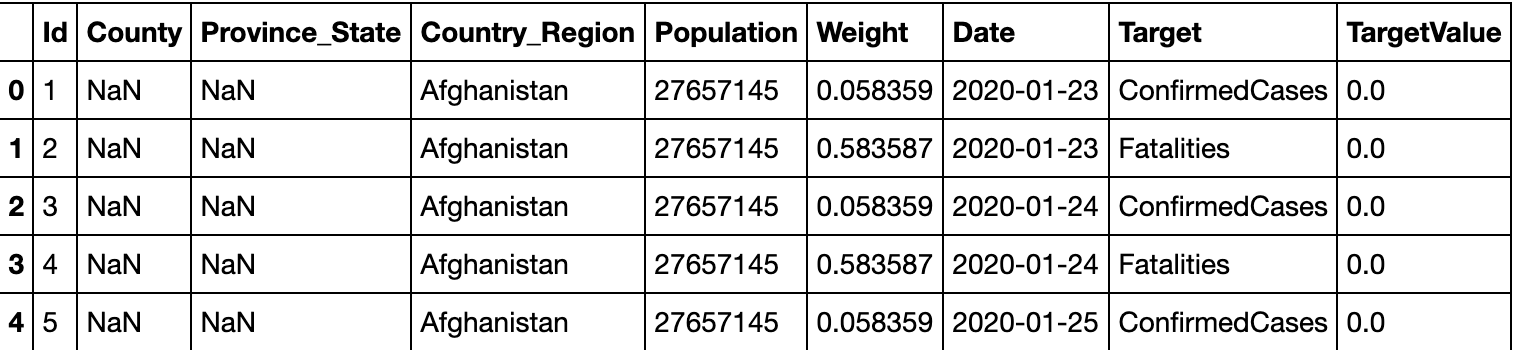
\includegraphics[width=\columnwidth]{train_head.png}
  \caption{Preview of first five line items in training dataset.}
\end{figure}

\begin{figure}
  \centering
  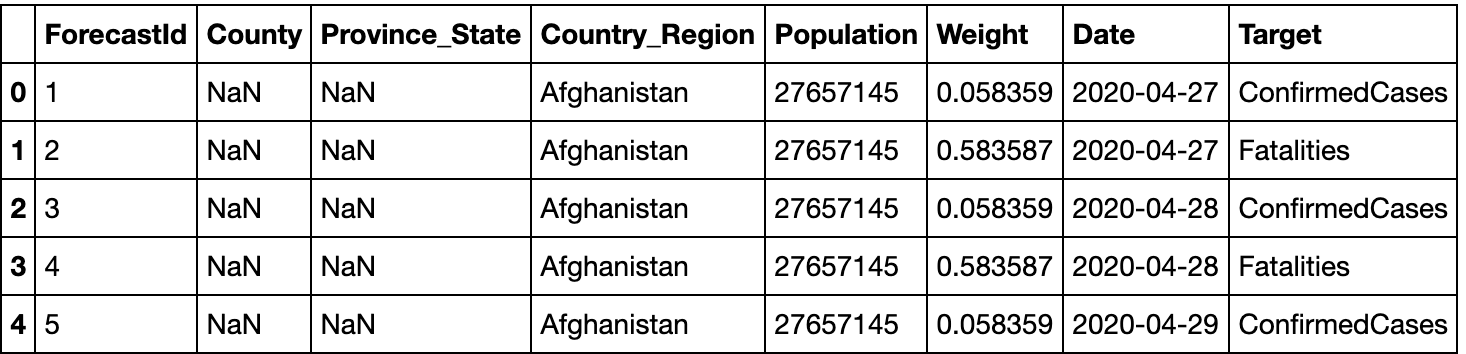
\includegraphics[width=\columnwidth]{test_head.png}
  \caption{Preview of first five line items in test dataset.}
\end{figure}
\begin{figure}
  \centering
  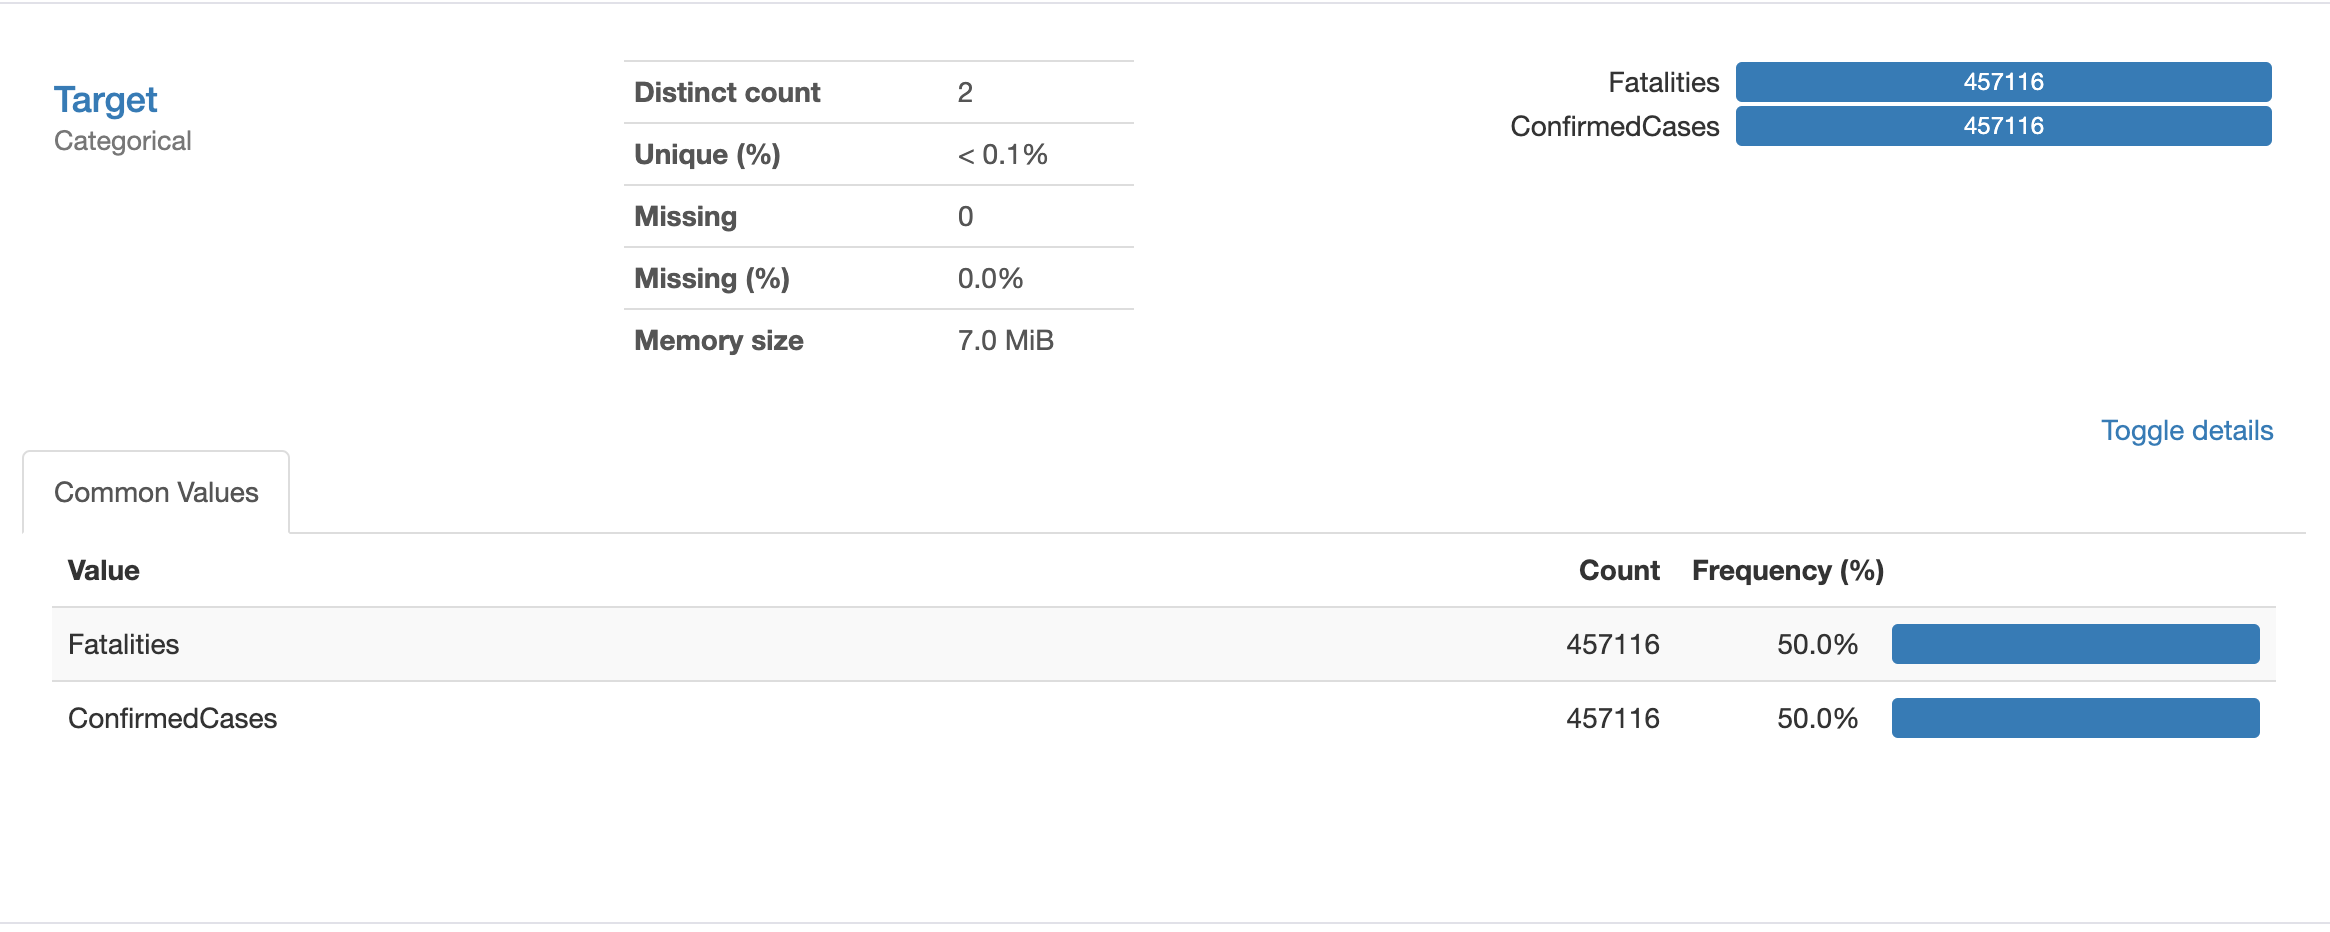
\includegraphics[width=\columnwidth]{target_values.png}
  \caption{Instances of confirmed cases and instances of fatalities.}
\end{figure}
\begin{figure}
  \centering
  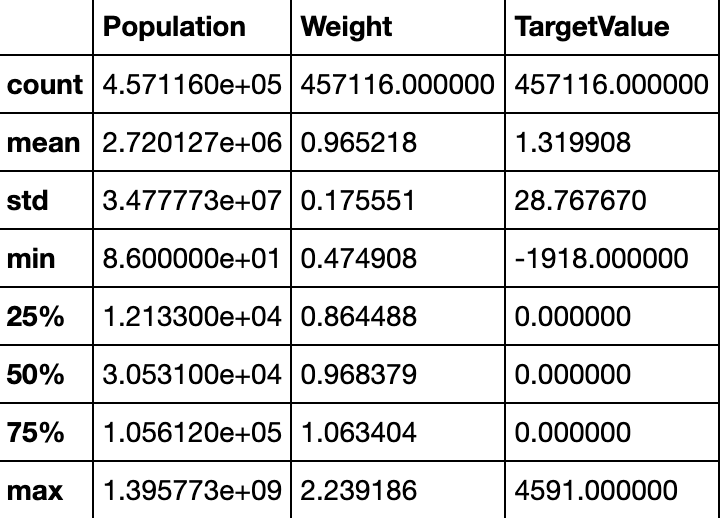
\includegraphics[width=\columnwidth]{fatalities.png}
  \caption{Summary statistics of fatalities.}
\end{figure}
\begin{figure}
  \centering
  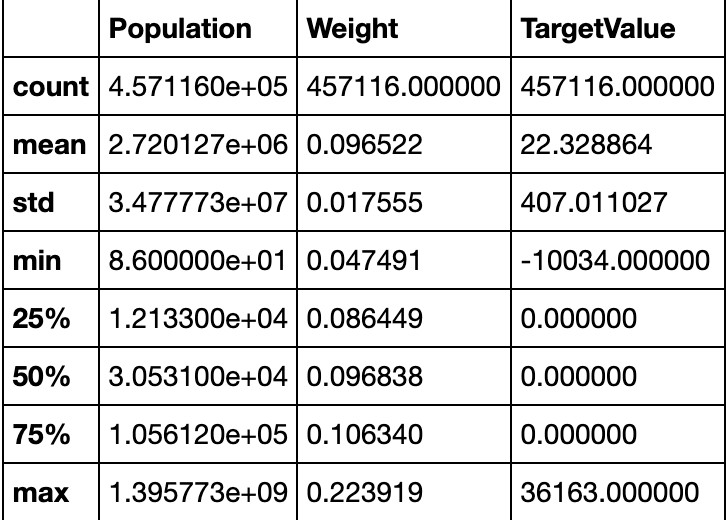
\includegraphics[width=\columnwidth]{confirmed_cases_summary_statistics.png}
  \caption{Summary statistics of confirmed cases.}
\end{figure}
\begin{figure}
  \centering
  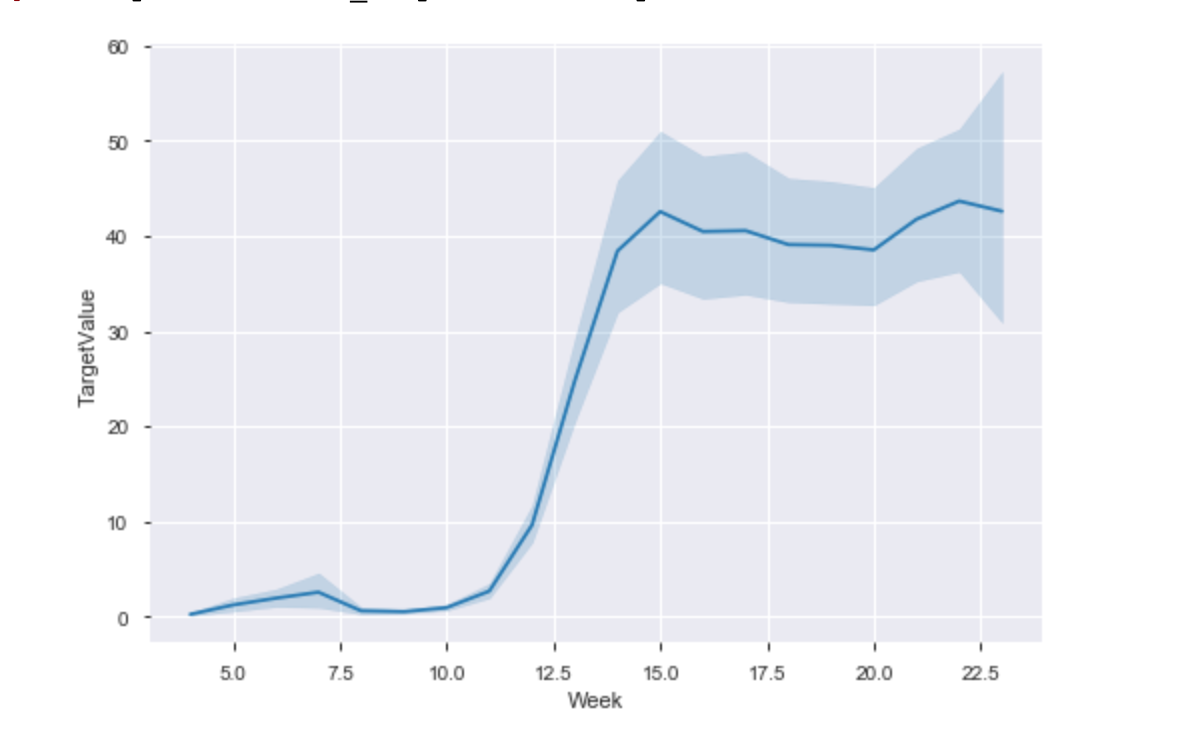
\includegraphics[width=\columnwidth]{week_vs_confirmed_cases.png}
  \caption{Number of confirmed cases by week.}
\end{figure}
\begin{figure}
  \centering
  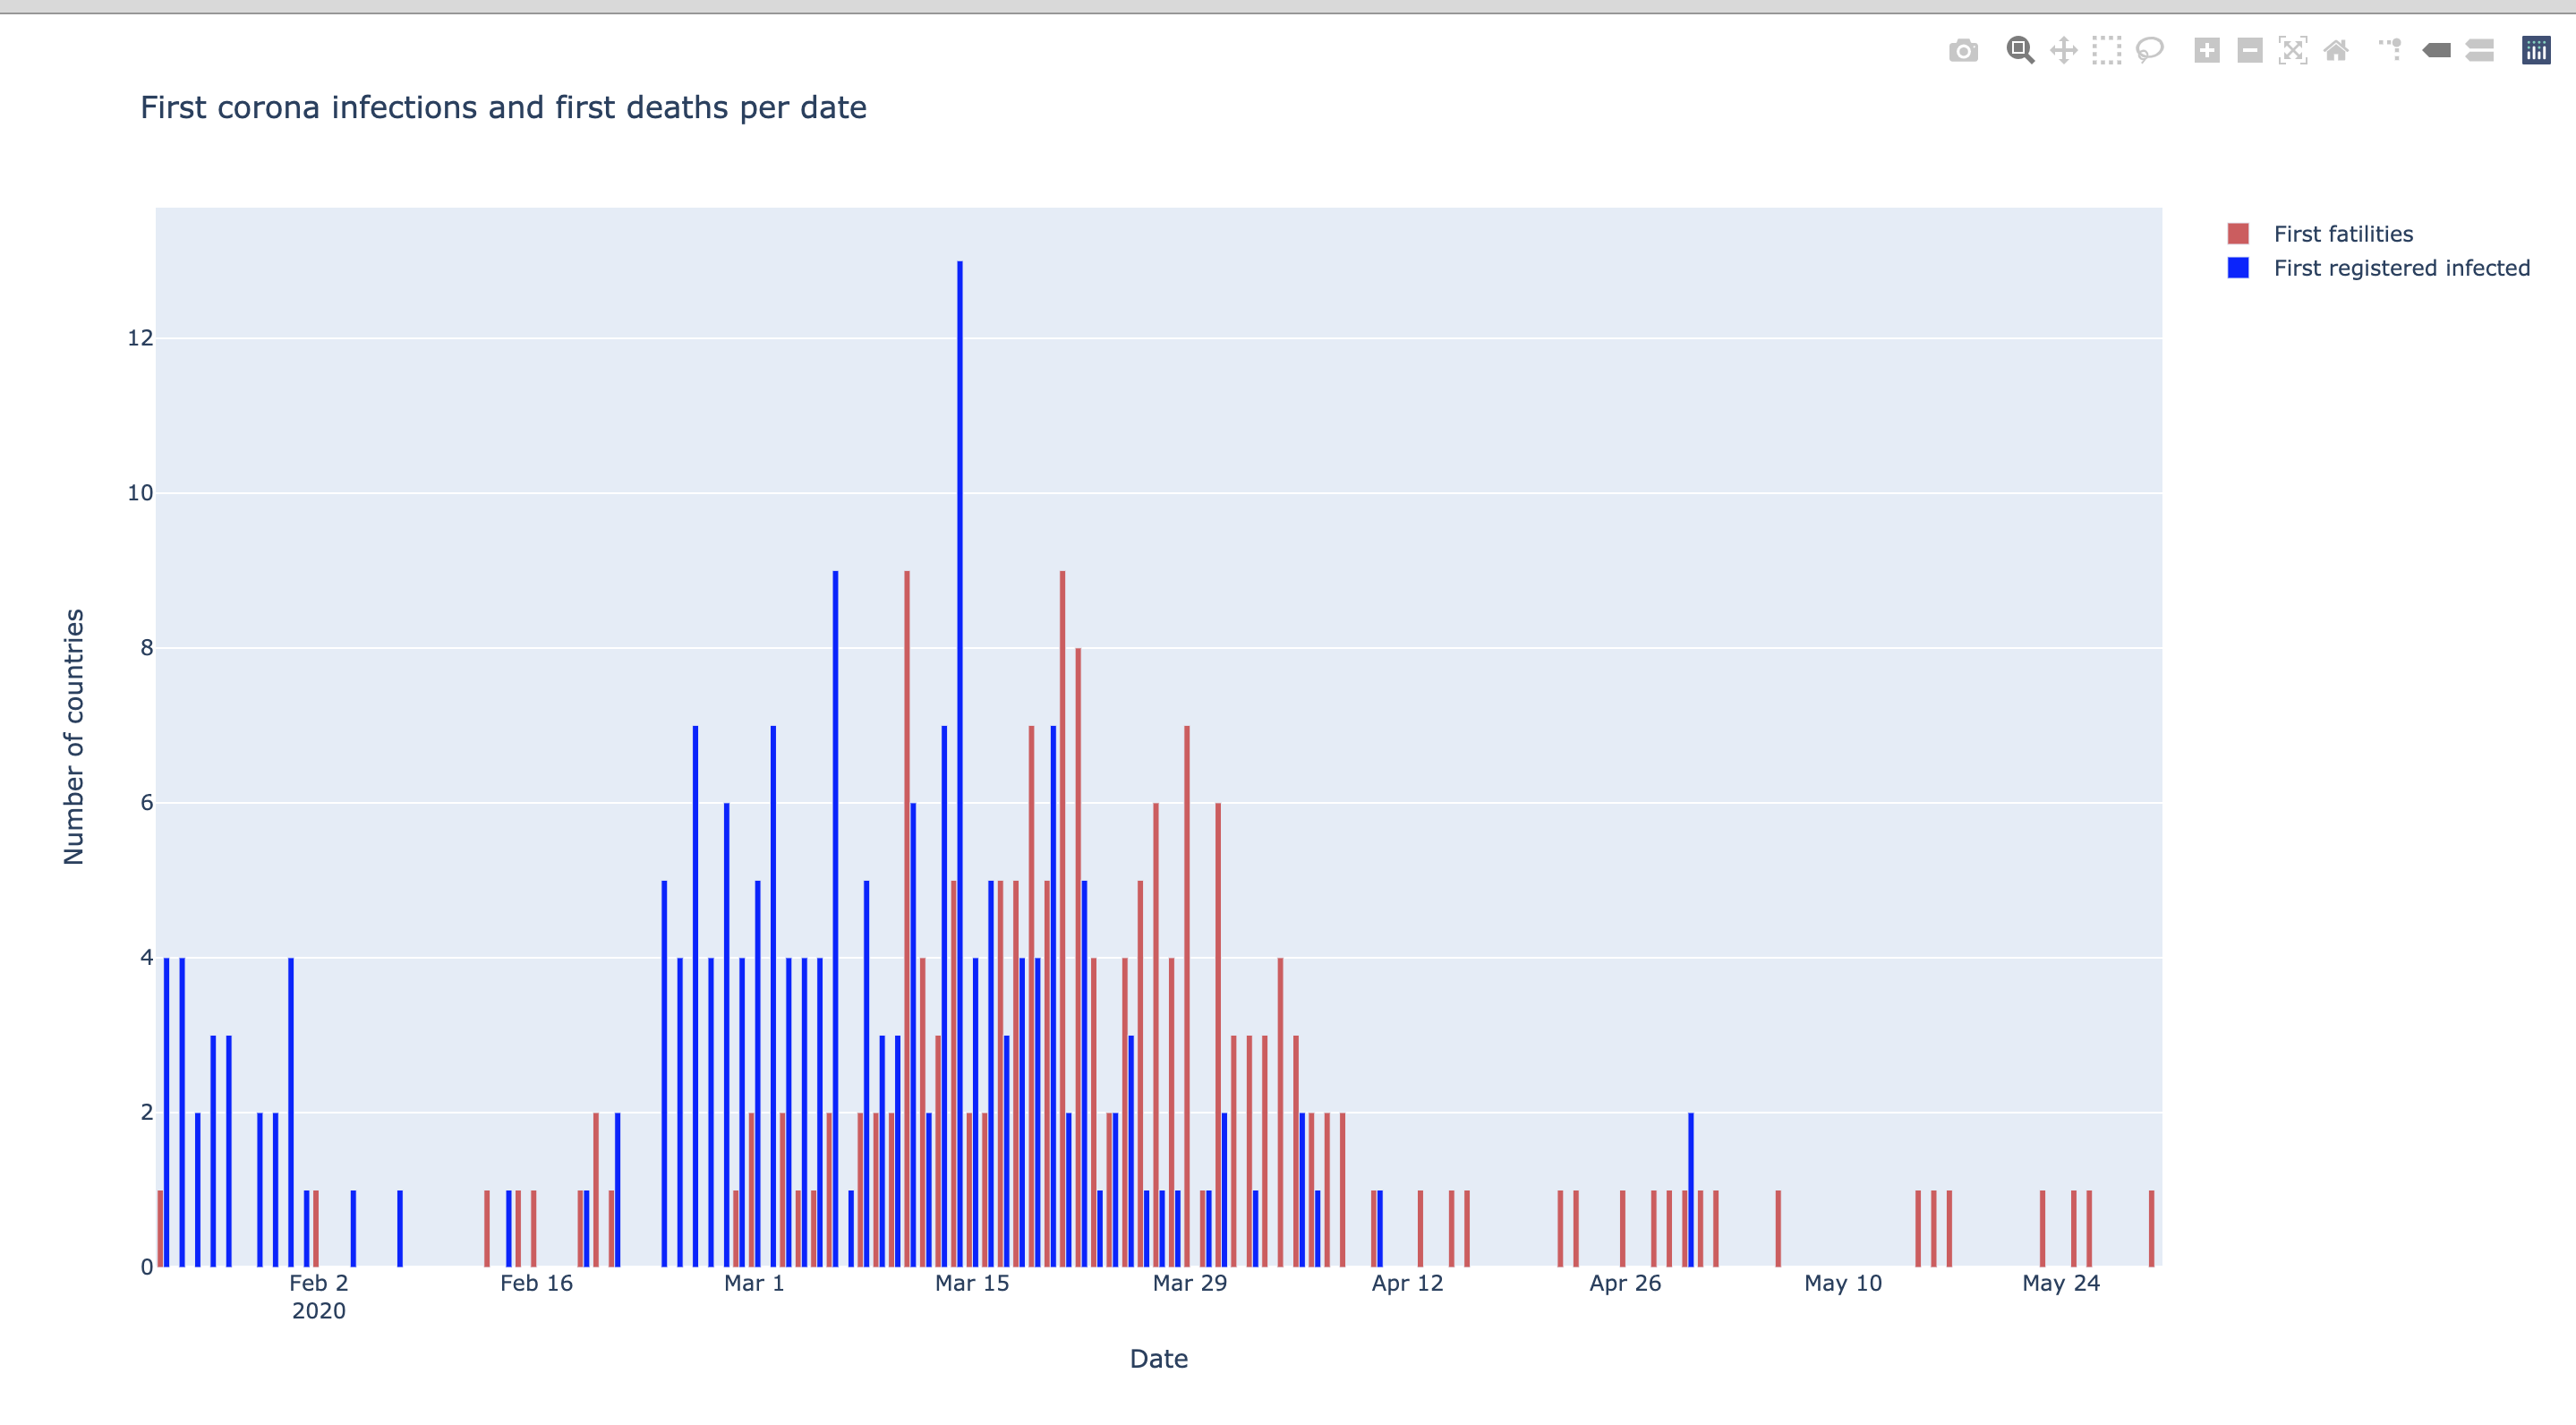
\includegraphics[width=\columnwidth]{first_infection_first_deaths.png}
  \caption{A distribution of first infections vs first deaths.}
\end{figure}

\begin{figure}
  \centering
  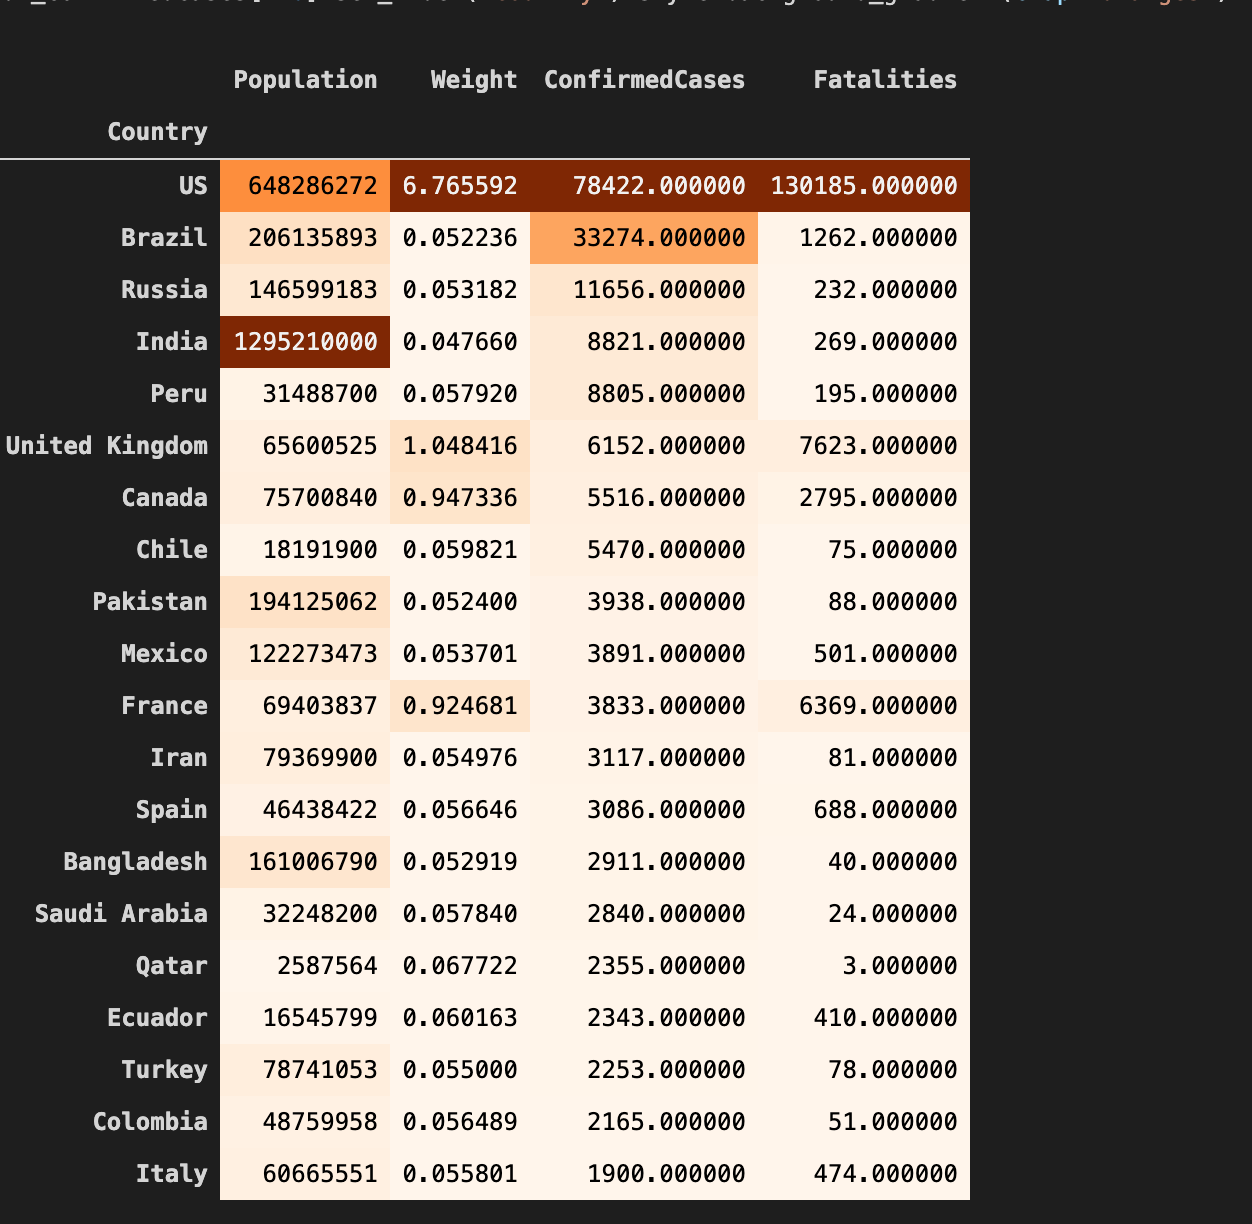
\includegraphics[width=\columnwidth]{covid_top_n_countries.png}
  \caption{Most inpacted countries.}
\end{figure}
\section{Methodology:}
\subsection{Data Cleaning:}
\begin{itemize}
\item We discovered negative values in the TargetValue field, for this reason we computed the absolute value for all TargetValues
\item We dropped all rows that had their Province\_State filled out. This was primarily due to the fact that this field was mostly set for a limited number of countries, such as $US$, $UK$ and $China$. This made the data skewed more towards American, United Kingdom and Chinese regions. 
\end{itemize}
\subsection{Data Enrichment:}
We obtained population by country \href{https://github.com/acquayefrank/MLDM2020-Project/blob/master/data/population_by_country_2020.csv}{data} and selected some fields to enrich our data.
We added the:
\begin{itemize}
  \item  population density
  \item  population median age
  \item  urban population  percentage
\end{itemize}
\subsection{Feature Engineering:}

To create a sufficient model it is of course important to give the model the best features to work with. As stated in a previous section, data on $Population density, Urban population and Median age$ was added. Also  it was chosen to treat the time-series data $Date$ as more numerical values. From the date the number of the week, the number of the day, the day in the week and the number of days since the first confirmed case(s) were derived. 
From Permutation importance and impurity based feature importance, stemming from $Random Forest Regressor$, it was found that these alterations indeed resulted in important features. In \emph{figure 11} and \emph{figure 12} we can find that the Permutation difference for the different datasets are fairly similar, although the feature for Population Density seems to be slightly more important in the fatalities dataset than in the confirmed cases dataset. 
The feature importances that were derived from the same $Random Forest Regressor$ look similar, however give less of an importance to the Country being the $US$. The plots for the feature importances can be found in \emph{figure 9} and \emph{figure 10}.

\begin{itemize}
\item We extracted the week from the date
\item We extracted the day from the date
\item We extracted the weekday from the date
\item We computed the date since the first infection was recorded in a country
\item We split our data into recorded fatalities and number of confirmed cases by day
\item We then did a one hot encoding for all countries listed in our data
\item We dropped the Id, County and Province\_State columns since we realised it negatively impacted predictions as depicted in \emph{Figure 9}. The feature Unnamed is the Id field
\end{itemize}

\begin{figure}
  \centering
  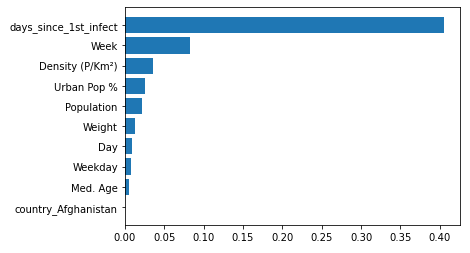
\includegraphics[width=\columnwidth]{feature-imp-f-randfor.png}
  \caption{Feature Importance for confirmed cases dataset after some experimental models were created (Random Forest).}
\end{figure}

\begin{figure}
  \centering
  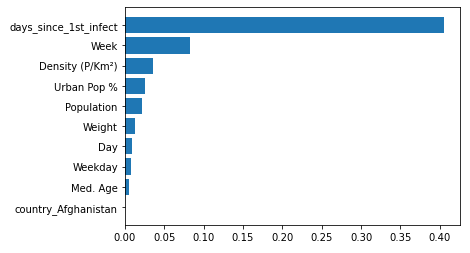
\includegraphics[width=\columnwidth]{feature-imp-f-randfor.png}
  \caption{Feature Importance for fatalities dataset after some experimental models were created (Random Forest).}
\end{figure}

\begin{figure}
    \centering
    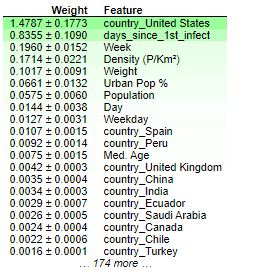
\includegraphics{feature-permutation-importance-cc-data.png}
    \caption{Permutation importance for confirmed cases dataset.}
\end{figure}

\begin{figure}
    \centering
    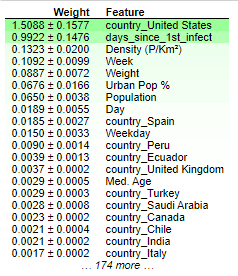
\includegraphics{feature-permutation-importance-f-data.png}
    \caption{Permutation importance for fatalities dataset.}
\end{figure}

\section{Experiment setup and results; error analysis:}
Our initial approach was to experiment with trees and obtain feature importance, then create regression models with these features. But during our experiments we realised trees performed better. More importantly ensemble learning methods performed better.
\\
\\
Since the official test dataset provided by Kaggle had no labels, we discarded that dataset and split our training data into test and training. We split the data based on date. All dates after `2020-05-20` were placed in our test data and dates after  `2020-05-20` were placed in training data.

As can be seen from the table, we have experimented with several models, to find that Tree-based ensemble methods perform best on this dataset. Therefore it was chosen to optimize those models. 

\begin{tabular}{ |p{5cm}||p{3cm}||p{5cm}|  }
 \hline
 \multicolumn{3}{|c|}{Model Analysis} \\
 \hline
 \hline
Model   & R2 Score & Comments\\
 \hline
 \hline
 Ridge Regression   & -404026.412 & Performs badly  \\
   \hline
 ElasticNet  & 0.079 & Relatively better than Ridge Regression \\
  \hline
   ExtraTreesClassifier & 0.217 & Relatively better than Ridge Regression \\
 \hline
  Linear Regression   & 0.475 & Relatively better than Ridge Regression \\
  \hline
SGDRegressor   & 0.518 & Relatively better than Linear Regression \\
  \hline
  GradientBoostingRegressor & 0.7979 &  One of our top 4 models \\
   \hline
  HistGradientBoostingRegressor & 0.862 &  One of our top 4 models \\
  \hline
  RandomForestRegressor & 0.892 &  One of our top 4 models \\
  \hline
   DecisionTreeRegressor & 0.899&  One of our top 4 models \\
  \hline
\end{tabular}

\section{Discussion:}

In this section the different models and their results, before and after hyperparameter optimization will be discussed. The models we have chosen to optimize were the models that in our initial test performed best. Interestingly, the four best performing models are all, but one, Tree-based Ensemble models. The Decision Tree Regressor is not an ensemble model, but it is a tree-based model. The ensemble technique combines predictions from several machine learning algorithms, in order to make more accurate predictions. 
The first two ensemble models we will discuss are Boosting models, which entails that each model that is build will learn which features to focus on from the previous model. 

\subsection{Gradient Boosting Regressor:}

Gradient Boosting is a method in which a prediction model is constructed as an ensemble of prediction models, often decision trees. In the sklearn implementation of this model a regression tree is fitted on a negative gradient, and aims to minimize the given loss function. 
This model performed decently on the default hyperparameters, achieving a $r2 score$ of $0.7979$ for both datasets. To optimize this model $Random Search$ was used, from different trials it came forth that best results come when leaving a large part of the hyperparameters on their default setting, but tuning the $learning rate$, $max depth$ and the $minimum samples per leaf$. The model achieved a $r2 score$ on the confirmed cases dataset of 0.8469 and on the fatality dataset of 0.8429. 

\subsection{Hist Gradient Boosting Regressor:}
The Hist Gradient Boosting Regressor is quite similar in its workings to the previously discussed model, it is however optimized for big datasets, where the number of datapoints exceed 10.000. 
It outperforms the normal gradient boosting regressor by 0.862 $r2 score$. This might be explained by the way this estimator splits and handles the data (as histograms instead of ordered features). 
After optimization of the hyperparameters the $r2 score$ is ...

\subsection{Random Forest Regressor:}
The Random forest is a technique where multiple decision trees are build, the predicted score (for regression) is often the mean prediction of all the individual trees. This ensemble model employs bagging technique, in which there is no interaction between the decision trees whilst building them. 
Random Forests are often praised for their robustness in comparison to a decision tree. 
On our datasets The Random Forest Regressor performs rather well, achieving a $r2 score$ of 0.892 on the confirmed cases dataset, with default parameters. After optimization of the following parameters we achieved an $r2 score$ of ...

\subsection{Decision Tree Regressor:}
Decision Trees are build in a tree structure, it breaks down a dataset into smaller subsets, where at each node a decision must be made. In our case a decision could look like: $Week <= 12$, after this decision the tree splits in subtrees. The more explanatory power a decision has, the higher up the decision will be in the tree. The most important decision node is call the root node. The mentioned explanatory power depends on the metric used, from the optimization we derive the $MSE$ is the best metric for this dataset. 
The Sklearn implementation of Decision Tree Regressor with default hyperparameters already gives rather good results with an $R2 score$ of 0.899. After hyperparameter optimization with Random Search the highest $R2 score$ achieved was ... 




\section{Conclusion:}
We realized esemble learning regressors performed better with the key feature being days since first infection was recorded in a country/region.
\end{document}
